%\documentclass[12pt,journal]{IEEEtran}
 \documentclass[12pt,journal,draftclsnofoot,onecolumn]{IEEEtran}
\IEEEoverridecommandlockouts
\usepackage{cite}  
\usepackage{amsmath,amssymb,amsfonts}
\usepackage{algorithm}
\usepackage{algorithmic} 
\usepackage{textcomp}
\usepackage{xcolor}    
\usepackage{amsthm}  
\usepackage{graphicx}
\usepackage{multirow}  
%\usepackage{algpseudocode}
\usepackage{booktabs}
 
\renewcommand{\algorithmicrequire}{\textbf{Input:}} 
\renewcommand{\algorithmicensure}{\textbf{Output:}} 
 
\def\BibTeX{{\rm B\kern-.05em{\sc i\kern-.025em b}\kern-.08em
		T\kern-.1667em\lower.7ex\hbox{E}\kern-.125emX}}

 
%\geometry{left=2.54cm,right=2.54cm,top=1.0cm,bottom=1.0cm}

\title{Adaptive Beam Scheduling for Cooperative Phased Array Radars with High-Precision Pencil-Beam}
\author{Anbang Deng, Ben Liu, Ratnasingham Tharmarasa, Thiagalingam Kirubarajan}
\date{}
\begin{document}
\maketitle

\begin{abstract}
Phased array radar (PAR) has attracted considerable attention in civil and military applications due to its capability to simultaneously perform multiple tasks. To make better use of limited radar resources and to offer best operating performance, an efficient resource allocation strategy is necessary. In this paper, two cooperative PARs with the capability of generating fan-beam and pencil-beam for search and track (SAT) functions in a finite time horizon, is assumed. In contrast to the traditional PAR scheduler, a pencil-beam with super narrow beamwidth cannot cover the whole area of interest, especially in the cases of maneuvering target with high motion uncertainty, resulting in potential missed detection in one beam scan. Our work addresses the problem of pencil-beam scheduling. In order to utilize the limited time and the energy resources, it is necessary to provide an efficient beam scheduling algorithm. However, the problem of scheduling both fan-beam and pencil-beam for perform SaT efficiently is barely discussed and addressed in literature. Aiming at above issues, two optimization models for the PAR task scheduling and a general solution based on hierarchical genetic algorithm (HGA) for the mixed  integer nonlinear problem (MINP)  are proposed.  The proposed mechanism implements the optimal resource allocation based on the feedback information from the trackers in order to maintain a reasonably low tracking accuracy. To handle the partially covered target existence area by pencil-beam, the predicted expected posterior Cramér–Rao lower bound (P-EPCRLB) is used as the main optimization criteria for the scheduling strategy.  In addition, by using a linear-wipe strategy,  we build another  PCRLB-based problem  optimization model with lower computational complexity. Numerical results demonstrate the superior performance of the proposed strategy and the effectiveness of the proposed solution.

    
\end{abstract}

\begin{IEEEkeywords}
Phased array radar, resource management, beam scheduler, narrow beam width, Posterior Cramér-Rao lower bound
\end{IEEEkeywords}


\section{Introduction}
\subsection{Background and Motivation}
Recent advancement in phased array technology enables the radar beams to be controlled and adapted almost instantaneously \cite{fenn2000development,van1993phased,orman1996scheduling}. The use of modern phased array antennas or electronically steered antennas (ESA) has enhanced the flexibility and effectiveness of radars by allowing them to swiftly switch among different tasks. These advantanges of phased array radars provide them with the capability to carry out multiple functions simultaneously, which typically include surveillance, tracking and weapon engagement.

The problem of resource management\cite{ding2008survey,moo2015adaptive,punithakumar2006multisensor,tharmarasa2007pcrlb,hero2011sensor,schmaedeke1993information} arises when a radar does not have sufficient resource to handle all tasks. An effective resoure management algorithm, therefore, is required to properly allocate limited radar resources to different tasks or to maintain the tracking error under a certain threshold. There are three major resources in a radar system: 1) \emph{time}: the most constraining resource that determines whether a task or function should be excuted or delayed. Correspondingly, numbers of typical resource management problems involve time allocation, such as task prioritization\cite{kuo2005real} and sensor scheduling\cite{narykov2013algorithm}; 2) \emph{power}: limited by overall power supply. The performance of a certain task is dependent on the power allocated to it, thus power allocation problems arise as to maximize the overall performance by efficiently allocating limited power to all tasks \cite{she2016novel,yan2015simultaneous}; 3) \emph{processing budget}: consumed by signal processing operations such as confirming or update tracks, limited by the capacity of computer processors\cite{tharmarasa2019closed}. These issues often appear as constraints (e.g., battery life) in resource management problems. In a more generalized sense, certain radar parameters that affect radar performances such as waveform or bandwidth, are also considered as special resources and need to be optimized during task execution.  Considerable efforts have been dedicated to the investigation of waveform design\cite{kershaw1994optimal} or bandwidth allocation\cite{paris2019genetic} and tracking update scheduling\cite{hong1998optimal}, in terms of radar resource managment.

Due to the broad definition of resource management problems, detailed mathematical modeling varies. Generally, radar resource management is treated as an optimization problem with a predefined criterion or objective function and several operational contraints. One typical criterion is quality of service (QoS)\cite{ghosh2006integrated}. QoS-based radar allocation model (Q-RAM) algorithms are defined to optimize the radar system to maintain an acceptable level of QoS. Q-RAM allows multiple QoS requirements such as timeliness, cryptography and reliable data delivery to be addressed and traded off against each other. In \cite{irci2010study}, Q-RAM for single and multiple resource types is comprehensively studied and a gradient projection algorithm is developed. 

Considerable efforts have been dedicated to the solution of resource management optimizations. Solution techniques can be preliminarily catagorized into AI approaches and non-AI approaches\cite{ding2008survey}. A recent research\cite{shaghaghi2018machine} proposed a machine learning-based branch-and-bound (B\&B) method to solve the NP-hard problem while maintaining a modest computational cost. In \cite{izquierdo1994optimal}, a neural network approach is adopted to solve the time scheduling problem of transmitting and receiving pulses. In \cite{miranda2007fuzzy,miranda2006knowledge}, a fuzzy logic method is  developed to determine the priority of tasks, and thereafter, allocate power to them. Rule-based heuristic searches, such as genetic algorithm (GA)\cite{zhang2019hybrid} or particle swarm optimization (PSO)\cite{zhang2011multiple} are also classified into this catagory.

Non-AI approaches include dynamic programming \cite{stromberg1996scheduling,castanon1997approximate,washburn2002stochastic} and convex optimization techniques \cite{boyd2004convex,li2020adaptive}.

Beam scheduling is a specific genre of radar resource management where one wishes to schedule the radar beams, i.e., determine the steering direction and operation time, to perform certain tasks. Additionally, power allocated to each beam and beam parameters, e.g., beamwidth, may also be considered as variables to be optimized. Recently, a task scheduling problem has been studied in \cite{zhang2019hybrid} and a hybrid adaptively genetic algorithm utilizing chaotic sequence is proposed that overperforms adaptive GA and high priority and earliest deadline first (HPEDF) algorithm.  

In real-life cases, radars may have flexible beam generation modes to satisfy different requirements. Pencil-beams with narrow width can provide measurements with high angle resolution and thus are preferred in high-precision tracking, while fan-beams with wide width are suitable to search for potential targets. Fig (\ref{fig:beams}) shows different beam generating of a PAR.
 
In the literature, it is usually assumed that the radar scan resolution cell size is large enough to cover the potential location of the targets\cite{hernandez2004multisensor,bar2004estimation}, hence, the beam steering problem coincides with the task scheduling problem where steering a beam to point at a certain target is equivalent to assigning the beam to that tracking task. However, for tracking highly maneuvering targets with pencil-beams, the previously stated assumption may not hold and it is not guaranteed that the target can be detected within one scan due to the small coverage size of the narrow beams. Thus, our interest is to develop an adaptive scheduling algorithm of narrow beams to make best use of limited resources and performance the best tracking performance. At each scheduling interval, the scheduler controls the radar beams to obtain the measurement data so that the tracking performance is maximized. Searching functions can be fulfilled using the gap time\cite{kang2004coordinated}.

\begin{figure}
	\centering
	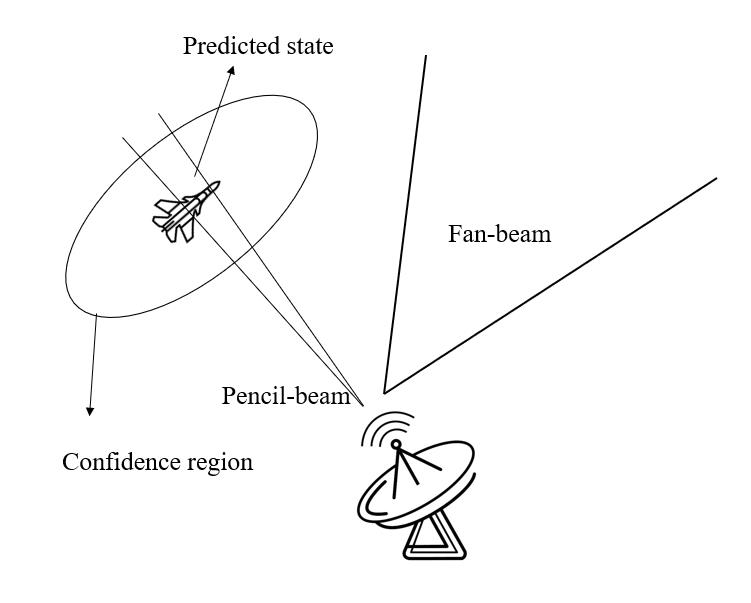
\includegraphics[scale=0.38]{Two Beams.jpg}
	\caption{Different beam modes}
	\label{fig:beams}
\end{figure}

Existing research on beam scheduling in terms of resource management mainly focus on normal-size beams to increase tracking accuracy, but narrow beams are barely considered. In practice, however, the adoption of pencil-beams is necessary when tracking with higher resolution is required. Furthermore, launching narrow beams is an effective and efficient method of resource allocation since it concentrates the power for beam generation. As narrow beams demonstrate great potentials in large-volume surveillance and highly maneuvering target tracking, the narrow beam scheduling problem is meaningful to address.  

The Posterior Cramér-Rao lower bound (PCRLB), given by the inverse of Fishcer Information Matrix, provides a lower achievable minimum of the estimation mean squared error (MSE) for any unbiased estimator\cite{tichavsky1998posterior}. \cite{niu2012target} states that the estimaion error asymptotically approaches the PCRLB in high SNR if the measurement noise is Gaussian. Hence, PCRLB is often used as a criterion to minimize. In the case of high-accuracy tracking with pencil-beams, the concept of expected PCRLB (EPCRLB) is proposed to handle the partial observations.

%In our work, we consider a cooperative radar system with a number of radar nodes. Each radar node launches a single pencil-beam for target tracking.


\subsection{Main Contributions}
In this paper, we intend to address the problem of narrow pencil-beam scheduling for cooperative phased array radars. All radar nodes in the system work in a cooperative fashion, where they share the measurement data together and make decisions on beam control. The information exchange among radar nodes will be fulfilled via wireless communication.

This paper makes the following contributions:

1) \emph{A new pencil-beam scheduling problem is addressed and formulated as an optimization problem.} Pencil-beams have narrow beamwidth so that they may not cover the entire area of interest. The scheduling problem of such narrow beams is firstly addressed and mathematically formulated as an optimization problem.

2) \emph{The concept of expected posterior Cramér-Rao lower bound (EPCRLB) is proposed and utilized as the criterion to minimize.} The PCRLB, which gives an achievable lower bound for any unbiased estimator, is utilized as the metric that needs to be optimized. However, due to partial observations obtained by pencil-beams, PRCLB cannot be obtained analytically. Therefore, the expected PCRLB that applies the idea of Monte Carlo trial is proposed.

3) \emph{An alternative linear wipe solution is proposed.} A target-driven solution that utilizes linear wipe strategy is proposed. It has less computational complexity and is shown to be effective while the maneuvering level of targets is low.

4) \emph{An ABS-based framework for multitarget tracking is developed.} An IMM algorithm is employed to handle maneuvering target tracking. The nonlinear filtering is dealt with by local UKF. A closed-loop signal processing framework is established for the radar system. Details of the framework is illustrated in Fig. 1.

\begin{figure}
	\centering
	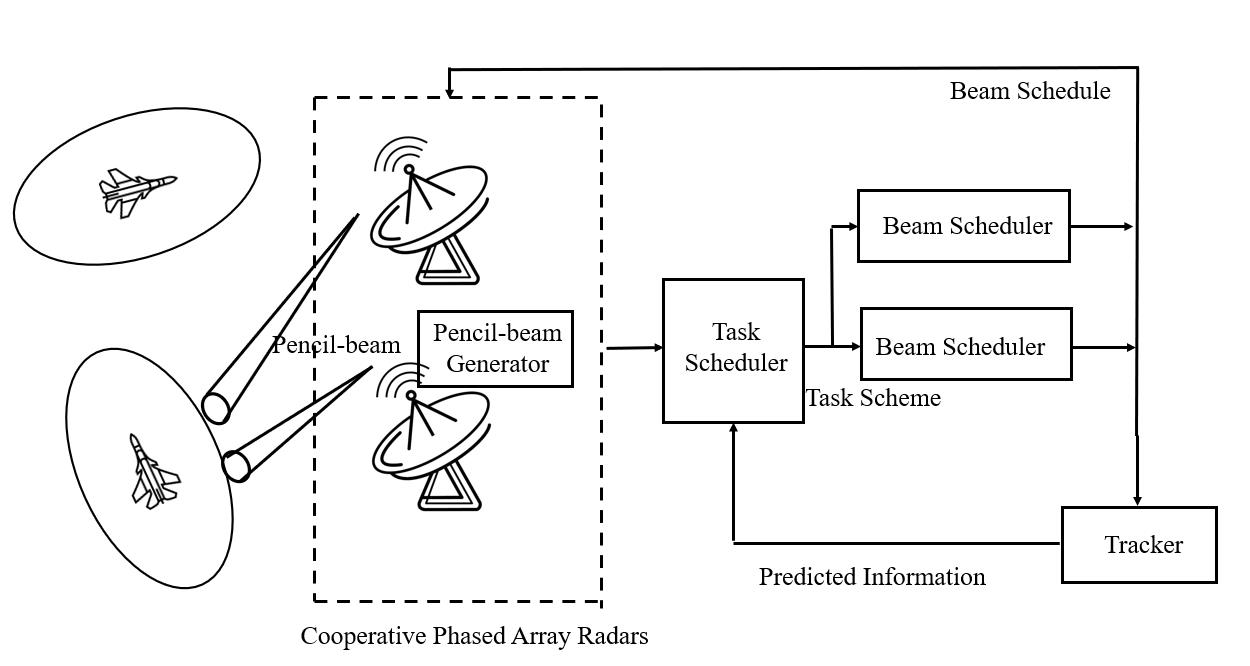
\includegraphics[scale=0.28]{Flow Chart.jpg}
	\caption{ABS-based multitarget tracking framework in a cooperative radar system}
	\label{fig:system}
\end{figure}

The remainder of the paper is organized as follows. Section II describes the problem and introduces preliminary knowledge. Problems formulations and corresponding soluton techniques are presented in Section III. Numerical simulations are demonstrated in Section IV and conclusions are given in Section V. 

\section{Problem Description}
For simplicity, we assume a 2-D surveillance area where a radar system with $N$ cooperative phased array radar nodes is deployed. The position of the $n$th node is denoted by $(x_{n},y_{n})$. There are $Q$ airborne targets to be tracked. The $q$th target is intially located at $(x_q^1,y_q^1)$ with an initial velocity $(\dot{x}_q^1,\dot{y}_q^1)$. At time step $k$, the $q$th target is located at $(x_q^k,y_q^k)$ with velocity $(\dot{x}_q^k,\dot{y}_q^k)$.

 The assumptions used to define the problem are as follows:
\begin{itemize}
	\item The radars can proveide a super narrow-width beam mode for high-accuracy target tracking. Such narrow pencil-beam cannot cover the entire confidence region of the target location.
	\item Each radar can only launch one single beam for target tracking.
	\item The number of radar nodes $N$ is smaller than the number of targets $Q$, i.e., there will always be targets that are not illuminated by any radar in each time step.
	\item The radars can switch the direction of their beams instantaneously.
	\item The number of targets is known and remains constant. All tracks are already confirmed.
\end{itemize}


\subsection{Target Dynamics}
\label{sec:target}
Let $\mathbf{x}_q^k={[x_q^k, y_q^k, \dot{x}_q^k, \dot{y}_q^k]^T}$ denote the state vector of the $q$th target, where $\left[ x_q^k, y_q^k \right]$ and $\left[ \dot{x}_q^k, \dot{y}_q^k \right]$ denote the position and velocity of the target, respectively.

The state space model that describes the $q$th target's motion is given by
\begin{equation}\ \mathbf{x}_q^{k+1}=\mathbf{F}_k\mathbf{x}_q^k+\mathbf{w}_q^k
\end{equation}

Where $\mathbf{x}_q^k={[x_q^k, y_q^k, \dot{x}_q^k, \dot{y}_q^k]^T}$ is the column state vector of the $q$th target, and $\left[ x_q^k, y_q^k \right]$ and $\left[ \dot{x}_q^k, \dot{y}_q^k \right]$ denote the position and velocity of the target, respectively. $\mathbf{F}_k$ denotes the state transition matrix. ${\mathbf{w}_q^k} $ is the process noise assumed to be the model input to control the evolution of target state ${\mathbf{x}_q^k}$. $\mathbf{w}^k$ is the process noise that describes the inaccuracy of the motion model. It is assumed to be zero-mean Gaussian distributed with a known covariance $\mathbf{\Gamma}^k$.

\begin{equation}
	{\bf \Gamma}_{k}=\kappa {\bf I}_{2}\otimes\left[\begin{matrix} {1\over 3}T^{3}&{1\over 2}T^{2}\\ {1\over 2}T^{2}&T\end{matrix}\right]
\end{equation}

where $\kappa$ is the intensity of process noise.

In this paper, we consider two target dynamic models: constant velocity (CV) and constant turn (CT) with a known turn rate.

For the CV model, the transition matrix is given by

\begin{equation}
    {\bf F}_k={\bf I}_{2}\otimes\left[\begin{matrix}1 & T \\ 0 & 1\end{matrix}\right]
\end{equation}

where $\otimes$ is the Kronecker operator, and $\mathbf{I}_2$ denotes the $2\times 2$ identity matrix. 

For the CT model, the transition matrix is given by

\begin{equation}
	{\bf F}_k=\left[\begin{matrix}1 & {\sin \omega T \over \omega} & 0 & -{1-\cos \omega T \over \omega} \\ 0 & \cos \omega T & 0 & -\sin \omega T \\ 0 & {1-\cos \omega T \over \omega} & 1 & {\sin \omega T \over \omega} \\ 0 & \sin \omega T & 0 & \cos \omega T\end{matrix}\right]
\end{equation}



%The transition model of the $i$th target is a first-order Markov process which is described as:
%\begin{equation}
%    \mathbf{h}_k^i=\mathbf{h}_{k-1}^i+\mathbf{\mu}_{k-1}^i
%\end{equation}

%The noise $\mathbf{\mu}_{k-1}^i$ is white Gaussian with a known covariance $\mathbf{Q}_{h,k-1}^i$. The term $\mathbf{h}_k^i=[\mathbf{h}_{1,i,k}^T,\mathbf{h}_{2,i,k}^T,...\mathbf{h}_{N,i,k}^T]^T$ represents the channel state vector ($\mathbf{h}_{j,i,k}=[h_{j,i,k}^R,h_{j,i,k}^I]^T$). Then, the system state vector is extended by concatenating the target state vector and the channel state vector.


\subsection{Measurement Model}
\label{sec:measurement}
We define a binary variable $o_{m,n,q}^k$ to indicate whether the $q$ th target is illuminated by the $m$th scan of the $n$th radar node at time step $k$. Failure to illuminate a certain target may be caused by task assignment schemes (as previously mentioned, there are always targets that are not tracked.) or missed detection due to partial observation. The measurement is given by:

\begin{equation}
    \mathbf{z}_{n,q}^k=\begin{cases} h_{n}(\mathbf{x}_q^k)+\mathbf{w}_{n,q}^k & \text{if}\ o_{m,n,q}^k=1\\ \mathbf{0}^k & \text{if}\ o_{m,n,q}^k=0
    	\end{cases}
    \label{measurement function}
\end{equation}

where $\mathbf{z}_{n,q}^k$ is the measurement of target $q$ at time step $k$ that is obtained by the $n$th radar, $h_{n}$ is the nonlinear observation function. Generally the measurements include range $R_{n,q}^k$ and bearing $\theta_{n,q}^k$:

\begin{equation}
	h_{n}(\mathbf{x}_q^k)=[R_{n,q}^k, \theta_{n,q}^k]^T
\end{equation}

Which are given by:

\begin{equation}
	\begin{cases}
		R_{n,q}^k= \sqrt{(x_{n,q}^k - x_n^k)^2+(y_{n,q}^k - y_n^k)^2} \\ 
		\theta_{n,q}^k=\arctan {(\frac{{y_{n,q}^k - y_n^k}}{{x_{n,q}^k - x_n^k}})} 
	\end{cases}	
\end{equation}

$\mathbf{v}_{n,q}^k$ is the measurement noise, which is assumed to be a zero-mean Gaussian random variable with covariance $\mathbf{\Sigma}_{n,q}^k$. 

\begin{equation} 
\boldsymbol {\Sigma}_{n,q}^k = \text{diag}\left({\sigma _{R_{n,q}^k}^2,\sigma _{\theta _{n,q}^k}^2} \right)
\label{measurement noise covariance}
\end{equation}

In practical scenarios, the probability of detection $P_d$ of each target is always less than unity due to the imperfectly interference. Besides, there exist false alarms over the surveillance area due to inevitable clutters. They are assumed to be a zero-mean Gaussian random variables uniformly distributed in the measurement space (within the observation volume $V$) with their number being a Poisson-distributed variable, given by 


\begin{equation}
	p(n_{fa})=\frac{e^{-\lambda V}(\lambda V)^{n_{fa}}}{n_{fa}!}
\end{equation} 

where $n_{fa}$ is the number of false alarms, $\lambda$ is the spatial density, i.e., the average number of false alarms at each frame.

\subsection{PCRLB and EPCRLB}
\label{sec:PCRLB}
The Cramér-Rao lower bound (CRLB), given by the inverse of Fischer information matrix (FIM), provides a lower bound of the error covariance matrix of any unbiased estimator for a certain parameter. The Posterior Cramér-Rao lower bound (PCRLB) gives a measure of the achievable accuracy for a dynamic state estimation. Since the PCRLB is irrelevant to the tracker, it is often adopted as a criterion to minimize in resource management problems. Let $\hat{\mathbf{x}_k}$ be an unbiased estimate of $\mathbf{x}_k$ based on the measurement $\mathbf{z}_k$, $\mathbf{C}_k$ be the error covariance matrix, and $\mathbf{J}(\mathbf{x}_k)$ be the FIM, we have 
\begin{equation}
    \mathbf{C}_k=\mathbb{E}[(\hat{\mathbf{x}}_k-\mathbf{x}_k)(\hat{\mathbf{x}}_k-\mathbf{x}_k)^{T}]\geq \mathbf{J}_(\mathbf{x}_k)^{-1}
\end{equation}

where $\mathbb{E}$ denotes expectation operator.

The FIM can be calculated with the following recursion\cite{tichavsky1998posterior}:

\begin{equation}
	\mathbf{J}_k=\mathbf{J}_X(\mathbf{x}_k)+\mathbf{J}_Z(\mathbf{x}_k)
	\label{J}
\end{equation}

$\mathbf{J}_X(\mathbf{x}_k)$ and $\mathbf{J}_Z(\mathbf{x}_k)$ are referred to as the prior knowledge and the measurement contribution at time step $k$, respectively.

\begin{equation}
	\begin{cases}
		\mathbf{J}_{X}(k)=\mathbf{D}_{k-1}^{33}-\mathbf{D}_{k-1}^{21}(\mathbf{J}_k+\mathbf{D}_{k-1}^{11})^{-1}\mathbf{D}_{k-1}^{12}\\
		\mathbf{J}_Z(k) =\mathbb{E}\{-\Delta _{\mathbf{x}_{k}}^{\mathbf{x}_{k}}\ln p(\mathbf{z}_k|\mathbf{x}_{k})\}
	\end{cases}    
\end{equation}

where
\begin{equation}
	\begin{cases}
		\mathbf{D}_{k-1}^{11}=\mathbb{E}\{-\Delta _{\mathbf{x}_{k-1}}^{\mathbf{x}_{k-1}}\ln p(\mathbf{x}_k|\mathbf{x}_{k-1}\}\\
		\mathbf{D}_{k-1}^{12}=\mathbb{E}\{-\Delta _{\mathbf{x}_{k}}^{\mathbf{x}_{k-1}}\ln p(\mathbf{x}_k|\mathbf{x}_{k-1}\}=(\mathbf{D}_{k-1}^{21})^T\\
		\mathbf{D}_{k-1}^{22}=\mathbb{E}\{-\Delta _{\mathbf{x}_{k}}^{\mathbf{x}_{k}}\ln p(\mathbf{x}_k|\mathbf{x}_{k-1}\}
	\end{cases}   
\end{equation}   

The prior information can be calculated by:
\begin{equation}
    \mathbf{J}_X(\mathbf{x}_k)=[\mathbf{\Gamma}_{k-1}+\mathbf{F}_k\mathbf{J}(\mathbf{x}_{k-1})^{-1}\mathbf{F}_{k-1}^T]^{-1}
    \label{eqn:Jx}
\end{equation}

The measurement contribution is given by
\begin{equation}
    \mathbf{J}_{Z_{n}}(\mathbf{x}_k)=\mathbb{E}\{\mathbf{H}_{q,k}^T\Sigma_{q,k}^{-1}\mathbf{H}_{q,k}\}
    \label{Jz}
\end{equation}

where $\mathbf{H}_{q,k}=[\Delta_{\mathbf{x}_q^k}h_n^T(\mathbf{x}_q^k)]^T$ is the Jacobian matrix of the measurement function $h_n(\mathbf{x}_q^k)$ with respect to the target state $\mathbf{x}_q^k$. and $\mathbb{E}$ denotes expectation with respect to the target state.

This expected value in (\ref{Jz}) cannot be obtained analytically. Approximcation is usually made by using the Jacobian and measurement noise covariance evaluated at the prediction phase to avoid extra computational cost.

\begin{equation}
	\mathbf{J}_{Z_{n}}(\mathbf{x}_k)=\mathbf{H}_{q,k}^T\Sigma_{q,k}^{-1}\mathbf{H}_{q,k}\bigg|_{\mathbf{x}_{k|k-1}^q}	
	\label{eqn:Jz}
\end{equation}

where $\mathbf{x}_{k|k-1}^q$ denotes the predicted state of the $q$th target at time step $k$. 


Note that in the calculation of $\mathbf{J}_{Z_{n}}(\mathbf{x}_k)$, an important assumption is that the target is scanned by the radar beam at time $k$ with a known target detection probability, false alarm rate and gating sizes. However, in the cases with narrow beam radar and target (i.e., drone) with high motion uncertainty, one beam scan will not be able to provide a full observation over the target, which makes the traditional PCRLB calculation be inapplicable. Here, an expected PCRLB (EPCRLB) is introduced to handle the partial observation problem. As the the calculation of $\mathrm{J}_{X}(k)$ in E-PCRLB is same to that in traditional PCRLB. Thus, only the new measurement contribution part denoted as $\mathrm{EJ}_{Z}(k+1)$ is detailed. $\mathrm{EJ}_{X}(k)$ is calculated based on the target existence density $\mathcal{D}_{t}$ (i.e., tracker outputs) and the angle coverage capability $\mathcal{C}_p$ of radar. Thus, one has
\begin{equation}
	\begin{aligned}
		&\text{E}\mathbf{J}_{Z_{n}}(\mathbf{x}_k)=\\
		&\int\limits_{\mathbf{x}_{k}\in \mathcal{C}_p}\mathcal{D}_{t}(\mathbf{x}_{k})\mathbb{E}\left \{{ -\Delta _{ \mathbf{x}_{k}}^{ \mathbf{x}_{k}}\ln p( {\mathbf{z}_{k}}| \mathbf{x}_{k}) }\right \} d\mathbf{x}_{k}
	\end{aligned}
	\label{EJZ_1}
\end{equation}
Note that the intersection of TED $\mathcal{D}_{t}$ and beam coverage $\mathcal{C}_{p}$ cannot be obtained analytically. Alternatively, the MC approach can be implemented. Thus, an artificial data set $\mathcal{S} $ of $\{\mathrm{ X}_k\}_{1}^{N_s}$is obtained from the TED. Next, an averaged PCRLB over the whole data set $\mathcal{S}$ is calculated with 
\begin{equation}
	\begin{aligned}
		&\text{E}\mathbf{J}_{Z_{n}}\approx\\
		&\frac{1}{N_s}\sum\limits_{{\mathbf{x}_{k}\in \mathcal{C}_p}\atop {\mathbf{x}_{k}\in \mathcal{S}}}\mathbb {E}\left \{{ -\Delta _{ \mathbf{x}_{k}}^{ \mathbf{x}_{k}}\ln p( {\mathbf{z}_{k}}| \mathbf{x}_{k}) }\right \} d\mathbf{x}_{k}
	\end{aligned}
	\label{EJZ_2}
\end{equation} 
where ${N}_s$ is the total number of points covered under one beam.

When the coverage of a single beam is larger than the target existence area and can provide a full observation of the target, the EPCRLB reduces to PCRLB.

The expression of EPCRLB has not been available before. And the EPCRLB is one of the critical formulations to address the measurement realization in CRLB and qualify the accuracy of target state estimates conditioned on the actual measurement realizations. Inspired by the ideas in\cite{song2010target}, the predictive EPCRLB (PE-PCRLB) is used by introducing the latest available measurement information to refine EPCRLB to formulate the {JBSA}  strategy for multitarget tracking in a multiple function phased array radar. 

\subsection{Cooperative multitarget tracking}
In this paper, a cooperative tracking is considered as opposed to independent tracking where tracks of a target are intialized and maintained separately by different radars. In a cooperative tracking framework, there is only one track for a single target. If there are more than one detection from multiple radars (or from false alarms), a detection-to-track data association is conducted\cite{moo2015coordinated}.

Since there are multiple models for target motion (\ref{sec:target}) and the measurement equations are nonlinear (\ref{sec:measurement}), IMM-UKF is used to handle the multitarget tracking. 

The IMM algorithm blends various motion models together to offer better tracking accuracy against maneuvering targets. In brief, IMM runs local filters for each model in the library and then evaluates the model probablity $\mu_{k}^{j-}$ at each time step. By combining all tracking outputs of different motion models, IMM can achieve proper tracking performance.

The updated state estimation is given by

\begin{equation}
	\hat{\mathbf{x}}_k = \sum_{j=1}^{J} \mu_{k}^{j-}\hat{\mathbf{x}}_k^{j}
\end{equation}

The updated covariance matrix is given by

\begin{equation}
	\hat{P}_k = \sum_{j=1}^{J} \mu_{k}^{j-}\{ \hat{P}_k^j +[\hat{\mathbf{x}}_k-\hat{\mathbf{x}}_k^{j}]\cdot[\hat{\mathbf{x}}_k-\hat{\mathbf{x}}_k^{j}]^T
	\}
\end{equation}

where $J$ is the number of motion models and $j$ is the model index.

Due to the nonlinearity of the measurement function (\ref{measurement function}), we use unscented Kalman filter (UKF) to fulfill the local filtering with one single motion model. Probabilistic data association (PDA) is used to handle measurement origin uncertainty arisen from missed detection and false alarms.
If a missed detection occurs when tracking a target, whether due to the partial observation or because this target was not assigned to any radar node, the tracker will simply predict the target's state and covariance and use them as the filter output. For more information about IMM, UKF and PDA, the reader is referred to \cite{bar2004estimation}.


\section{Beam Scheduler for Cooperative Phased Array Radar}
In this section, we intend to give detailed mathematical formulations of the beam scheduling problem. Sections \ref{sec:beam1} to \ref{sec:beam3} present three mathematical modeling and corresponding solution techniques. Section \ref{sec:complexity} gives the complexity analysis of these schedulers.

 
\subsection{Beam Scheduler 1: Fixed Linear Wipe}
\label{sec:beam1}
Since pencil-beams with small beamwidth cannot cover the entire area of interest, a straightforward solution is to consecutively and rapidly scan a position of potential target existence and its adjacent cells\cite{knott2012radar}. If the radar scans the area in a linear fashion, such technique is referred to as linear wipe.

Before scheduling precise beam steering directions, the radar system will roughly assign tracking tasks to each node with the task scheduler.

Let $A$ be the radar-to-target assignment matrix, such that 

\begin{equation} 
	A=\begin{bmatrix} a_{11} & & a_{1Q}\\ & \ddots & \\ a_{N1} & & a_{NQ} \end{bmatrix}_{N\times Q}  
\end{equation}

where $a_{n,q}$ takes value $1$ if the $q$th target is assigned to the $n$th radar and $0$ otherwise. Since every radar will be assigned to a tracking task, $A$ satisfies $\sum_{n\in R}a_{n,q}=1$.

To meet the requirement of tracking accuracy, the radar-to-target task assignment is completed by maximizing the worst-case PCRLB.

\begin{equation}
	\text{argmin}~\text{max}~ \{\text{PCRLB}_{n,q}\}, n=1,\cdots,N, q=1,\cdots,Q
\end{equation}

where $\text{PCRLB}_{n,q}$ is the PCRLB of the $n$th radar estimating the $q$th target. Since it depends on the Jacobian matrix which is relevant to the target's state, the PCRLB is evaluated with the predicted state $\mathbf{x}_k^-$ at time $k$. 

\emph{Remark 1:} The diagonal elements of the PCRLB matrix directly give the lower bounds of the squared estimation errors. Therefore, the trace of the PCRLB matrix is often used as a scalar characteristic while evaluating PCRLB. As an alternative, the sum of the first and the third diagonal elements, which represents the lower achievable squared errors of target position estimation, can be used for evaluation.

The PCRLB is calculated as 

\begin{equation}
	\text{PCRLB}_q = \mathbf{J}_X^q + \sum_{n\in \mathcal{N}}\mathbf{J}_{Z_n}^q
\end{equation}

where $\mathcal{N}$ is the set of radars that are assigned to target $q$. Note that during the task scheduling phase, multiple radars may be assigned with the same tracking task. $\sum_{n\in\mathcal{N}}\mathbf{J}_{Z_n}^q$ is the sum of measurement contributions obtained by all the radars tracking target $q$. As mentioned before, a coordinated tracking framework is used where there exists one single track for each target. If there are multiple detections from different radars, a detection-to-track data association is performed.

\emph{Remark 2:} Although it is possible that a single tracking task is assigned to multiple radar nodes, this situation does not commonly happen unless one target's motion uncertainty is significantly greater than the others'. Beside the data association technique, one can handle the issue of overlapped task by giving the current task only to the radar that provides the most measurement contribution $\mathbf{J}_Z^q$ and assigning other radars with different tasks. In this case, the overall estimation errors for multitarget tracking will be reduced.


Without loss of generosity, we can assume that the target does not move too much during $N_s$ successive tracking scans. During a tracking task, one wants to use $N_s$ scans on a target with predicted state $\mathbf{x}_k^{-}$ and predicted covariance $P_k^{-}$. Firstly, we compute the mean $m_k$ and  covariance $R_k$ in the polar measurement space with unscented transform (UT), shown as Fig. \ref{fig:UT}. UT handles the nonlinear mapping from target state to sensor measurement\cite{bar2004estimation}.

\begin{figure}
	\centering
	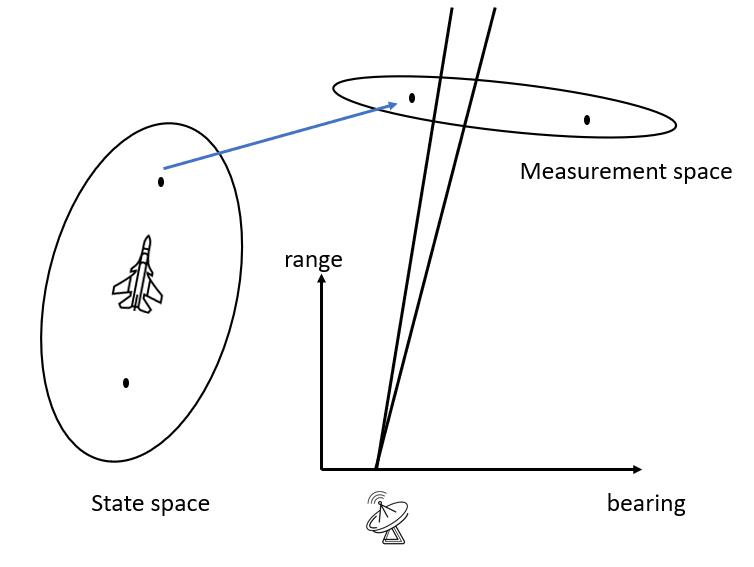
\includegraphics[width=3.5in]{UT.jpg}
	\caption{Unscented transform}
	\label{fig:UT}
\end{figure}


 Using a gating technique, one can determine the range of bearing around $m_k$. For simplicity, the range information is ignored here. In Fig. \ref{fig:linearwipe}, $c0$ is the value of bearing from the $m_k$, where the target exist with highest possibility. $cl_i,cr_j$ are the bearing cells on the left and right sides of the mean bearing value. Note that the cell size here is $\theta_{\text{track}}$. Let $N_s=18$, then we have a sequence of scans as the pattern below
 
 \begin{equation}
 	c0, cl_1, cr_1, cl_2,cr_2,cl_3,cr_3,cl_4,cr_4,cr_5,c0, cl_1, cr_1, cl_2,cr_2,cl_3,cr_3,cl_4
 \end{equation}
 
 One can compute the effective $\bar p_d=1-\prod_{s=1}^{S}(1-p_g^sp_d)$\cite{bar2004estimation}, where $S$ denotes the number of times where the radar covers the covariance area, here $S=2$. One can see that for 2nd scan, radar cannot guarantee a full $p_g$.
 
\begin{figure}
	\centering
	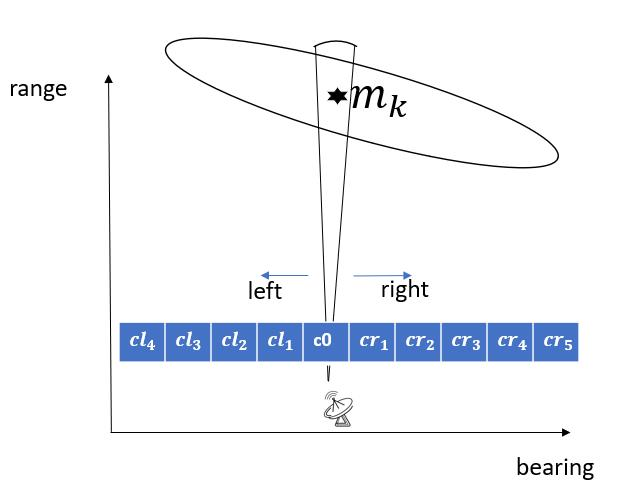
\includegraphics[width=3.5in]{Linear Wipe.jpg}
	\caption{Linear wipe}
	\label{fig:linearwipe}
\end{figure}


\emph{Remark 3:} The number of scans $N_S$ is determined by the total time of the mission interval. The total scan width for a batch scan (in the previous example, 10 cells) is determined by both the width of the target distribution (along the bearing direction) and the beamwidth. The radar will continue scanning linearly until the beam reaches the edge of the gate or until all scans have been used.

\subsection{Beam Scheduler 2:Open-loop Linear Wipe}

With the fixed scanning pattern, one can easily use linear wipe to fulfill tracking tasks. However, the size of the target spatial existence area will change during the surveillance period and its shape is dependent on the target-sensor geometry. Therefore, the fixed linear wipe will not satisfy our needs. Fig. \ref{fig:linearwipefails} shows a scenario where the target's existence area is small and only limited scans are required to track this target. With the fixed linear wipe strategy, the radar will continue to scan the area repeatedly while these scans could be allocated to other targets.

Herein, we develop an open-loop linear wipe solution that allocates tracking scans accordingly based on the specific target distribution $P_k^-$. Note that there is no task scheduling module before the beam scheduler. The evaluation of PCRLB, which is accomplished by the task scheduler, is incorporated in the beam scheduling process here.

\begin{figure}
	\centering
	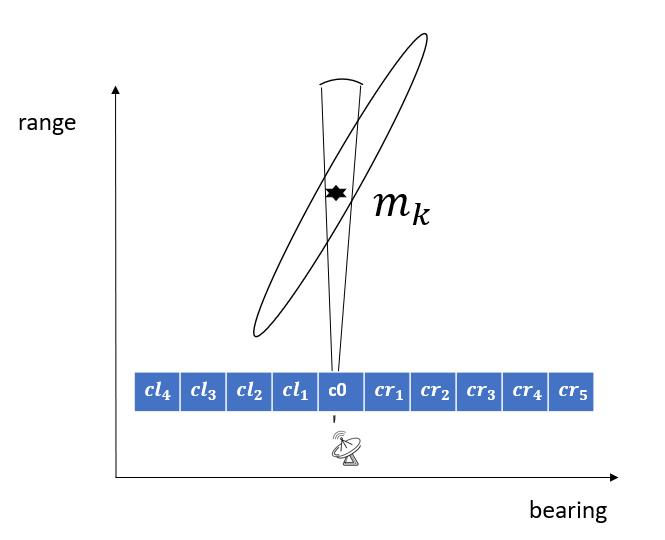
\includegraphics[width=3.5in]{Linear Wipe Fails.jpg}
	\caption{A target with small existence area}
	\label{fig:linearwipefails}
\end{figure}

Assume that $N_s$ scans is allocated for target $q$ at time $k$, then the radar will scan the area of interest from centroid to the edge successively. The unknown variables are 
\begin{equation}
	\begin{aligned}
		&\{(M_S, N_S)\},~~M_S\le N_S\\
		&\{(\text{ID}_1,N_s,t)_1,(\text{ID}_5,N_s,t)_i,\cdots,(\text{ID}_{N_t},N_s,t)_{i+n},(\text{ID}_{N_t-4},N_s,t)_{i+1+n},(\text{ID}_3,N_s,t)_{M_S}\},
	\end{aligned}
\end{equation}
where $\text{ID}_i$ is the identity index of each target, $N_{s,m}$ is the number of scans on each $\text{ID}_i$target within $m$th batch scan, and $N_t$ is the total number of targets in that time window. With this output, one can determine the scan order over all these targets and how much time is allocated for each of them for each batch scan. Note that $M_S$ determine the size of the sequence and $N_S = \sum_{m=1}^{M_S}N_{s,m}$ denoting the total number of tracking scans costed in this mission interval. The total number of scans should be less than the restricted value from the duty cycle. $0\le N_{s,m}\le N_S$, $t_{\text{start,plan}}\le t_m\le t_{\text{start,plan}}+t_{\text{plan}}$. $\sum_{m=1}^{M_S}N_{s,m} = N_S$.

\paragraph{Objective functions}
In this study, our aim is to provide a feasible beam scheduler that can aid the tracker with minimum track drops and errors and resources (time). To achieve the goal, multiple objectives are adopted.
\begin{itemize}
	\item Accuracy:
	\begin{equation}
		\text{argmin}~\text{max}~ \{\text{tr}(\text{PCRLB}_{i,t^{-}_{\text{scan}}})\}, i=1,\cdots,N_t, t^{-}_{\text{scan}}\in(t_{\text{start,plan}}, t_{\text{start,plan}}+t_{\text{plan}}]
		\label{eq::pcrlb_obj}
	\end{equation}
	where $\text{PCRLB}_{i,t^{-}_{\text{scan}}}$ is the $\text{PCRLB}$ matrix of target $i$ at time  $t_\text{scan}$ without update.
	\item Maximum average probability detection
	\begin{equation}
		\text{argmax}~\text{min}~ \{\frac{1}{\bar{N} _i}\sum_{m=1}^{M_S} \text{O(m,i)}\bar{p}^{m}_{d}\}, i=1,\cdots,N_t
		\label{eq::pd_obj}
	\end{equation}
	\begin{equation}
		\bar{N} _i =  \sum_{m=1}^{M_s}\text{O(m,i)}{N_{s,m}}, i=1,\cdots,N_t 
		\label{eq::numofscans_obj}
	\end{equation}
	\begin{equation}
		\bar p^m_d=1-\prod_{i=1}^{I_{m}}(1-p_g^{i} p_d)
		\label{eq::newpd}
	\end{equation}
	where $\bar{N}_i$ is the total number of batch scans over a single target. Using this objective function, one want to guarantee a good probability of detection (maximum $p_d$).
	\item Measurement contribution (Reward):
	\begin{equation}
		\text{argmax}~\text{min}~ \{\sum_{m=1}^{M_S} \text{O(m,i)}\mathbf{J}_Z^{m,i}\}, i=1,\cdots,N_t
		\label{eq::Jz_obj}
	\end{equation}
	where $\text{O}(s,i)$ equals One or Zero depending whether or not the target $i$ is illuminated by $s$th batch scan.
	\begin{equation}
		\mathbf{J}_Z^{m,i} = \bar{p}^m_d*\mathbf{J}_Z^i
	\end{equation}
	
	Where $I_{m} = \text{ceil}(N_{s,m}/{\hat N_{g,m}})$, where $\text{ceil}(\gamma)$ returns the smallest integer value that is bigger than or equal to a number $\gamma$, and $\hat{N}_{g,m}$ is minimum number of scans that one needs to get a full $p_g$ at $m$th batch scan. $\hat{N}_g$ varies with the state of target, size of covariance (mainly on bearing and elevation directions). From \eqref{eq::newpd}, one can increase the practical $\bar{p}_d$ infinitely close to One when $\hat{N}_g<<N_{s,m}$.
	As mentioned above, the value of $p_g^{i}$ is determined by the size of area of interest scanned within $m$th batch scan. For the cases in Figure \ref{fig:linearwipe}, with a full $p_g=0.95$, one have $S = 2$, $p_g^1 = 0.95$ and $p_g^2 = 0.8*0.95$
	
\end{itemize}
\paragraph{Optimization method}
The optimization problem is a mixed-integer nonlinear programming (MINLP). It combines both mixed-integer programming and nonlinear programming, which is NP-hard. To meet the real-time requirements, a fast method is needed. Herein, a hierarchical genetic algorithm is used.

\begin{figure}[H]
	\centering
	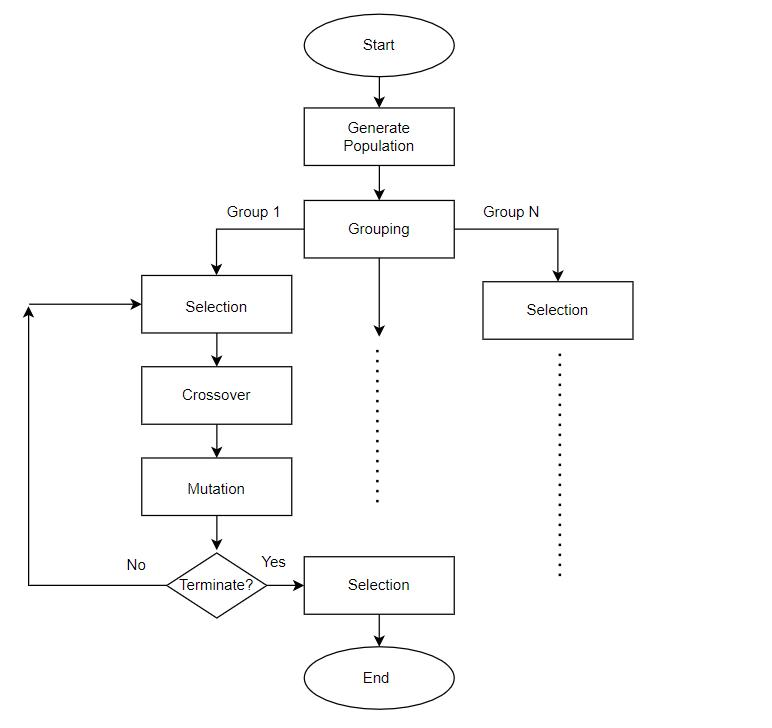
\includegraphics[width=3.5in]{GA.jpg}
	\caption{Hierarchical genetic algorithm}
	\label{fig:ga}
\end{figure}

Genetic algorithm (GA) is a heuristic searching technique that imitates the process of natural selection. Feasible solutions to the optimization problem are represented as individuals (also referred to as chromosomes) and are searched in a parallel manner that is called generations. In each generation, the fitness value of each individual is evaluated and then a selection operation is conducted. Individuals with high fitness value are more likely to be reproduced to the next generation while those with low fitness will be eliminated. Common selection techniques include roulette wheel and tournament selection. In this work, we adopt a binary tournament selection strategy.

To maintain the diversity and prevent early-maturing, crossover and mutation operations are performed. In a crossover operation, a locus is randomly chosen and the genes before and after this locus between two parent chromosomes are exchanged. In a mutation operation, each gene has a probability $P_m$ to be replaced by a random value.

Elitism is adopted in this paper to prevent the loss of highly fitted individuals. After each selection, few individuals with highest fitness values will be directly copied into the next generation without participating in the crossover and mutation operation. 

In our optimization problem, the length of chromosomes is determined by the number of batch scans $M_S$, thus individuals that represents diverse $M_S$ values will have different chromosome length. Chromosomes with different length cannot crossover with each other. Therefore, we apply a hierarchical genetic algorithm herein. Hierarchy refers to the presence of modules at multiple levels. Its basic idea is to group individuals with similar characteristics and have them evolve independently within their own group. In our MINLP, the structure of chromosomes is hierarchically divided into two different gene sequences that control $M_S$ and $n_S$, respectively. The entire popultion is split into several groups based on their $M_S$ value. Within each group, the individuals evolve independently and a best one will be found. Then, a global optimum is found among all groups by comparing their local optimum. The flow chart of HGA is presented in Fig. \ref{fig:ga}. 

\subsection{Beam Scheduler 3: EPCRLB-based optimal solution}
\label{sec:beam3}
In previous sections, it is assumed that the mobility of one target is low compared with the speed of tracking scans. This assumption might hold in some cases, but it is clearly not an optimal solution for narrow beam schedulling problem. Therefore, an optimal open-loop beam scheduler is proposed which considers the target motion characteristics into the formulation.


\paragraph{Objective functions}
In literature \cite{tharmarasa20,punithakumar2006multisensor,hernandez2004multisensor} and the method we proposed in Section \ref{sec:PCRLB}, the predictive {PCRLB} is utilized, where the $\mathbf{J}_Z$ can be computed as (\ref{eqn:Jz}).

Note that $\mathbf{J}_Z$ is determined by the predictive target state $\mathbf{x}_k$ with a fixed state of sensor $x_n$, which is valid as they assume that the one can cover the area where target potentially exists with one scan or multiple combined scans\cite{song2010target}. However, in practical cases with narrow beam scan, this assumption can no longer hold due to low coverage of the beam scan compared with the target localization uncertainty as discussed in Section \ref{sec:PCRLB}. Thus, an {EPCRLB} is proposed and adopted for the objective formulation. {EPCRLB} is calculated based on the target localization distribution and the scan capability of radar. With a set of state vectors $\mathbf{x}^m_k$, covariance matrices $P^m_k$ and corresponding weight values $w^m_k$, $m=1,\cdots,M$, one can formulate a target localization distribution. However, it is hard to analytically calculate the possible states covered by one beam scan. Here a number of particles extracted from the distribution are used to represent all the potential target states, which can be used to calculate the {EPCRLB}. As shown in Figure \ref{fig::epcrlbparticles}, a set of particles ${\xi_{p,i}}, i=1,\cdots, N_p$(black points) are extracted from two Gaussian distributions with known mean, covariance and weights. All the red points represents the part of target existence that are illuminated by radar. $\bar O(i)$ denotes whether or not that one point $\xi_{p,i}$ is included inside the scan area. Using \ref{eqn:Jz}, we have 
\begin{equation}
	\text{Jz}(\xi_{p,i}) = \text{E}[H_k(\xi_{p,i})R_s^{-1}H_k(\xi_{p,i})']
\end{equation}
Then the expected measurement contribution from this scan is given by 
\begin{equation}
	\text{E}\mathbf{J}_Z = \frac{p_d\bar{p}_gp_n}{\hat{N}_p}\sum_{i=1}^{N_p}\bar{O}(i)\mathbf{J}_{Z_i} 
\end{equation}
and $\bar{p}_g\approx \frac{\hat{N}_p}{N_p}p_g$, where $N_p$ is the toltal number of points used to represent the distribution, $\hat N_p$ is the number of points covered by one scan beam, and $p_n$ is the rate value that the new particles from $\hat{N}_g$ excluding already scanned particles before current scan. 

To make the problem clear, one simple example is illustrated here. As shown in Figure \ref{fig::targetmotion_pg_pn}, we use 9 particles to represent the target existence distribution, and 3 scans are included. At time $k-2$, one scan the central part of the area of interest and 6 out 9 particles are illuminated. As we assume this is the first scan, so $p_n=1$ as all the particles are scanned for the first time. Then, at time $k-1$, there is a new covariance matrix from the propagation of the target state. The beam moves to leftmost and 6 particles are scanned again but 3 of them are scanned twice, thus we have $p_n = 3/6$. For the current scan that illuminates the rightmost part of the area, 3 totally new particles are included, thus we again get $p_n=1$. From the process in the figure, one can see that $p_n$ denotes how much new information you can get from the scan compared with recent historical scans. This parameter $p_n$ controls the radar to go though the area of interest instead of only focus on the subregion providing highest $\mathbf{J}_Z$. Without using the $p_n$ in the formula, the radar might always want to point to the central part around the mean target state (shown as the red rectangle in Figure \ref{fig::targetmotion_pg_pn}) as it provides the higher $p_g$. Although it will return a high reward, the other region with high target existence possibilities are ignored, which may result in missed detections, especially for the scenarios with highly maneuvering targets. This is a new problem arising from narrow beam scheduling as only a small section of the area of interest can be covered with one single scan, thus in this study, we have to find a good combination of scans to not only increase the tracking accuracy but also the target detection possibility.


Thus, the expected {FIM} is given by 
\begin{equation}
	\text{E}\mathbf{J} = \mathbf{J}_X + \text{E}\mathbf{J}_Z
\end{equation}

where $\mathbf{J}_X$ is calculated as (\ref{eqn:Jx}).

\begin{figure}
	\centering
	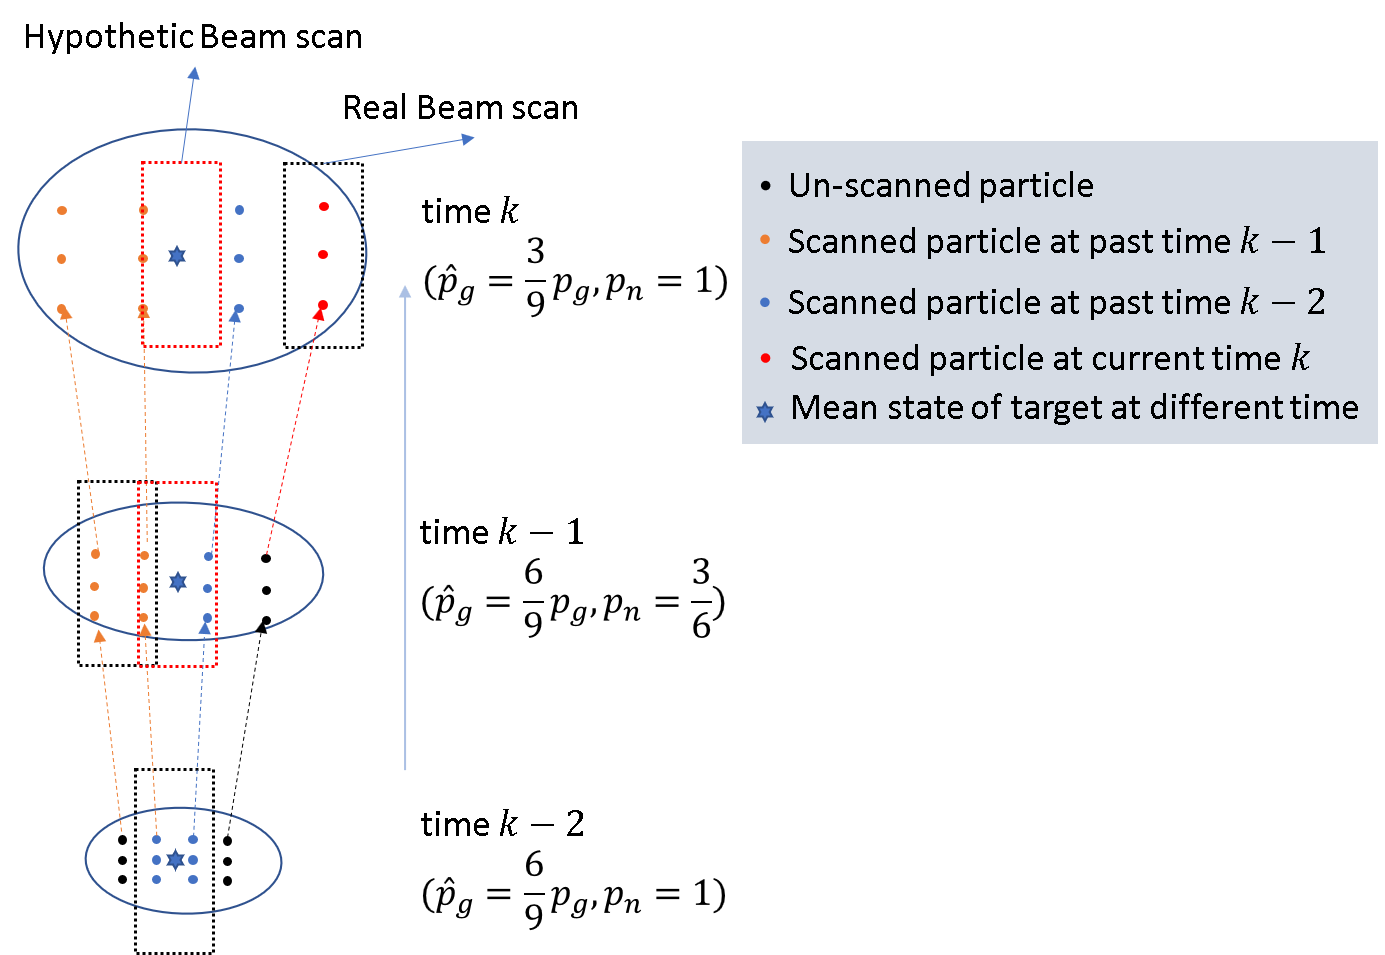
\includegraphics[width=3.5in]{targetmotion_pg_pn.png}
	\caption{targetmotionpgpn.}
	\label{fig::targetmotion_pg_pn}
\end{figure}
In this study, our aim is to provide a optimal beam scheduler that can aid the tracker with minimum track drops and errors and resources (time). To achieve this goal, multiple objectives are adopted.
\begin{itemize}
	\item Accuracy:
	\begin{equation}
		\text{argmin}~\text{max}~ \{\text{EPCRLB}_{i,t}\}, i=1,\cdots,N_t, t\in(t_{\text{start,plan}}, t_{\text{start,plan}}+t_{\text{plan}})
		\label{eq::pcrlb_objoptimal}
	\end{equation}
	\item Measurement contribution (Reward):
	\begin{equation}
		\text{argmax}~\text{min}~ \{\sum_{s=1}^{N_S} \text{O(s,i)} {\text{E}\mathbf{J}_Z}_{s,i}\}, i=1,\cdots,N_t
		\label{eq::Jz_objoptimal}
	\end{equation}
	where $\text{O}(s,i)$ equals One or Zero depending on whether or not the target $i$ is illuminated by $s$th single narrow beam scan.
	\item Number of scans (Cost)
	\begin{equation}
		\text{argmin}~\text{max}~ \{\sum_{m=1}^{M_s}{O}(s,i)\}, i=1,\cdots,N_t 
		\label{eq::numofscans_objoptimal}
	\end{equation}
	where $\bar{O}(s,i)$ equals to One or Zero depending if the target $i$ is illuminated or not. It can be determined using gating technique.   
\end{itemize}

\begin{figure}[H]
	\centering
	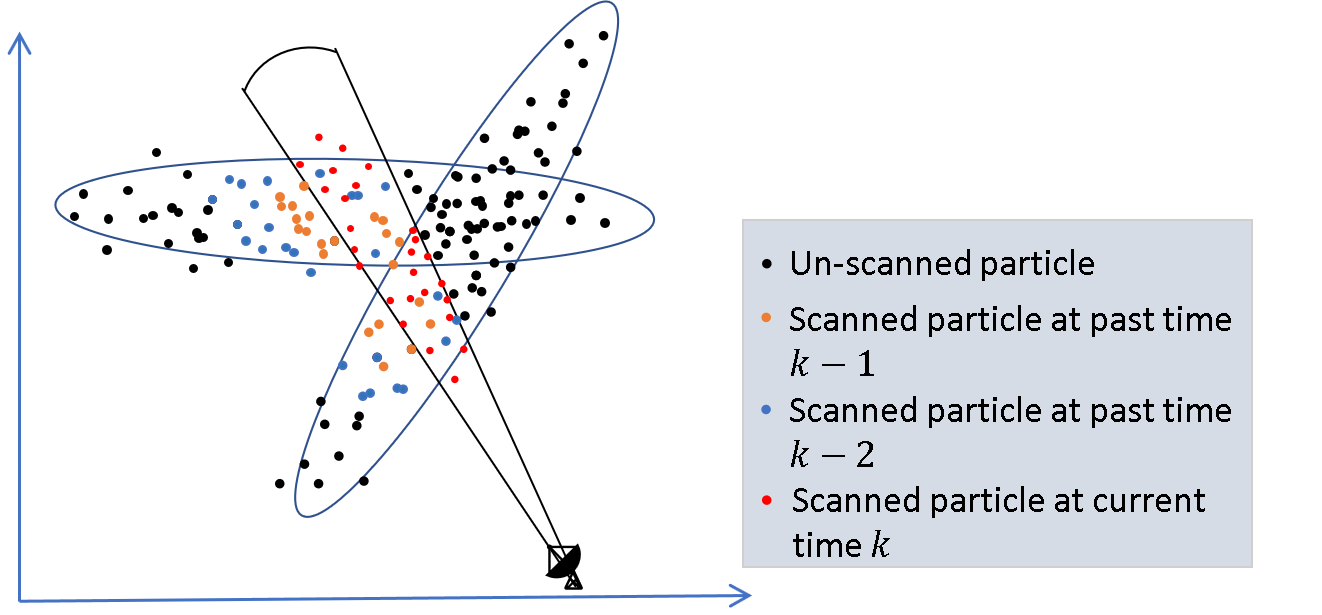
\includegraphics[width=3.5in]{epcrlbparticles.png}
	\caption{Conditional Jz.}
	\label{fig::epcrlbparticles}
\end{figure}

\subsection{Complexity Analysis}
\label{sec:complexity}
The complexity of the task scheduler incorporated in beam scheduler 1 is $\mathcal{O}(Q\times N)$. The search volume is enlarged when the number of radar nodes and/or targets is increased. The beam scheduler itself does not consume much computational budget, once the target existence area is calculated, the scanning pattern can be obtained.

The complexity of beam scheduler 2 is on the order of $\mathcal{O}(N_{pop}^1\times N_{pop}^2)$, where $N_{pop}^1$ and $N_{pop}^2$ are the population size of the first and the second level, respectively. $N_{pop}^2$ is independent of the problem size while $N_{pop}^1$ is propotional to the value of $Q\times N$. With the increase of the problem size, more combinations of radar-to-target assignment need to be investigated. The complexity of beam scheduler 3 is on the order of $\mathcal{O}(Q\times N\times N_p/\beta)$, where $N_p$ is the number of particles that represent the distribution of \emph{each} target and $\beta$ is the beamwidth. When $\beta$ is large enough to cover the whole area of interest, beam scheduler 3 reduces to a normal-beam scheduling strategy. 


\section{Simulation}
In this section, numerical results are presented to demonstrate the performance of the proposed strategies. Assume a phased array radar system with $N=2$ radar nodes is tracking $Q=3$ airborne targets. The radar nodes are located at $(-10,5)$ km and $(5,-10)$ km, respectively. The area is surveilled for 50 frames with the time interval $\Delta T = 1$s. The targets' motions are modelled by two dynamic models: constant velocity (CV) model and constant turn (CT) model with the turn rate known. Each target will perform two turing maneuvers during the surveillance period. The detailed information of targets is provided in Table \ref{tab:Target State} and their trajectories are shown in Fig. \ref{fig:Trajectories}. The beamwidth of the pencil-beam is set to $\beta=0.15^\circ$.

\begin{table}
	\centering
	\caption{Initial Target States}
	\begin{tabular}{ccccccc}
		\toprule
		Target Index & Position (km) & Velocity (m/s) & Turning Interval 1 & Turn Rate 1($^\circ$) & Turning Interval 2 & Turn Rate 2($^\circ$) \\ \midrule
		1 & (30,35) & (-200,-250) & (10,20) & 3 & (35,45) & -3\\ 
		2 & (-40,25) & (300,0) & (5,20) & 4 & (25,35) & 2\\ 
		3 & (-25,-20) & (100,25) & (10,15) & -4 & (35,45) & 5\\ 

		\bottomrule
	\end{tabular}
	\label{tab:Target State}
\end{table}  

\begin{figure}
	\centering
	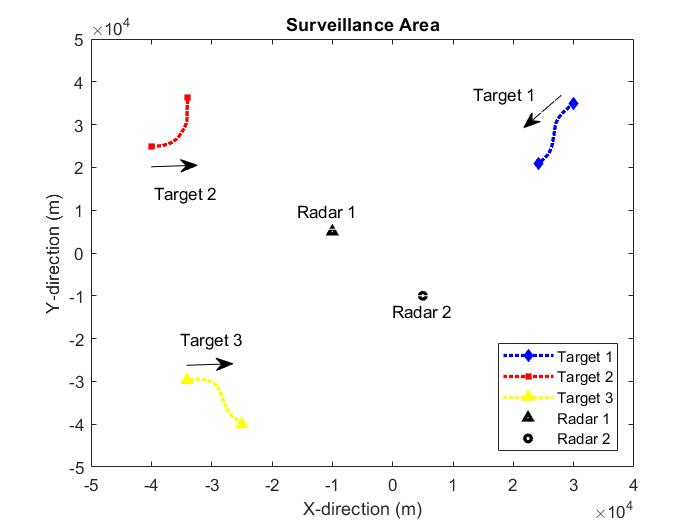
\includegraphics[scale=0.36]{Trajectories.jpg}
	\caption{Target trajectories and radar deployment}
	\label{fig:Trajectories}
\end{figure}

For the hierarchical cooperative GA used in the beam schedulers, the number of groups (first-level population size) is 15. Each group has 101 individuals. The probabilities of crossover $P_c=0.6$ and the probability of mutation $P_c=0.6$. Each group stops evolving once it reaches the maximum iteration 30 or there is no improvement within the latest 5 generations. For the optimal beam scheduler, each target's distribution is represented by $N_p=500$ particles. All results are averaged over 100 Monte Carlo runs.

\subsection{Comparison among ABS Strategies}
From Fig. \ref{fig:Worst PCRLB}, we can find that there are no significant differences among the worst-case PCRLB offered by three algorithms, although the optimal beam scheduler obtains a slightly lower PCRLB. Detailed data is given in Table \ref{tab:PCRLB all}. Note the bold numbers, the optimal solution already gives a lower PCRLB for target 1 though it doesn't change the worst-case PCRLB. This is because the worst-case PCRLB comes from the target that is not tracked.

 \begin{figure} 
	\begin{minipage}[t]{0.5\linewidth} 
		\centering 
		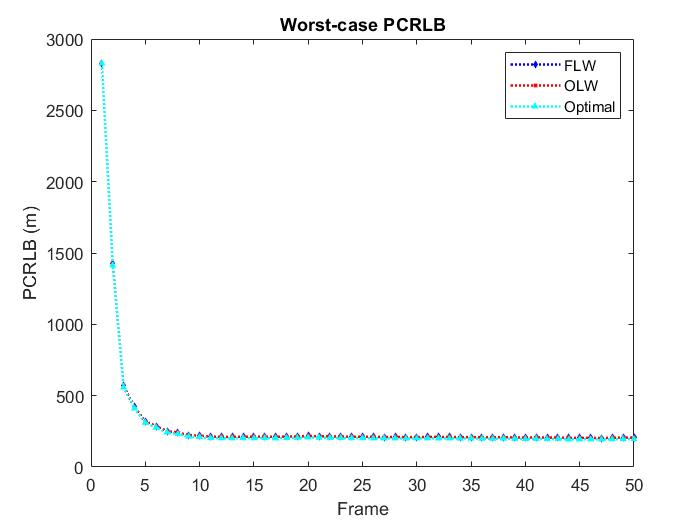
\includegraphics[scale=0.34]{Worst PCRLB.jpg} 
		\label{Path} 
	\end{minipage}% 
	\begin{minipage}[t]{0.5\linewidth} 
		\centering 
		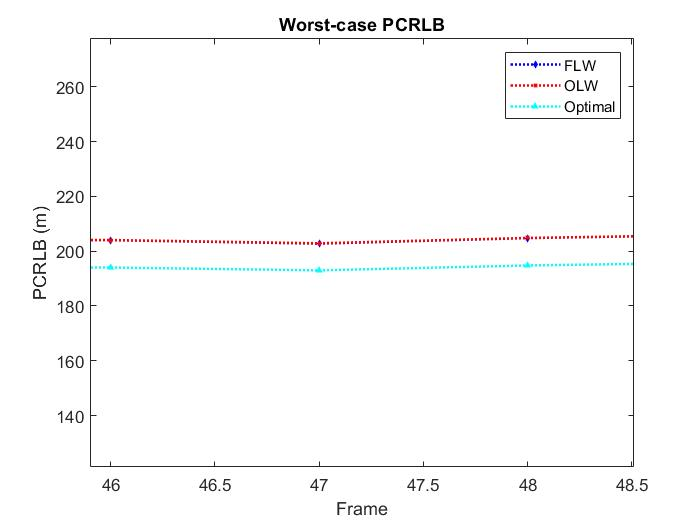
\includegraphics[scale=0.34]{Worst PCRLB_large.jpg} 
		\label{Power} 
	\end{minipage} 
\caption{Worst-case PCRLB}
\label{fig:Worst PCRLB}
\end{figure}

\begin{table*}
	
	\centering
	
	\caption{PCRLB of Each Target}
	
	\begin{tabular}{cccccc}
		\toprule
		\multirow{2}{*}{Time Index}&
		\multirow{2}{*}{Algorithm}&
		\multicolumn{3}{c}{PCRLB of Target No.}&\multirow{2}{*}{Worst-case PCRLB}\cr
		\cmidrule(lr){3-5}
		&&1&2&3\cr
		\midrule
		\multirow{3}{*}{2}&FLW&693.6&1424.2&558.5&1424.2\cr
		\cmidrule(lr){2-6}
		&OLW&693.6&1424.2&558.5&1424.2\cr
		\cmidrule(lr){2-6}
		&Optimal&693.6&1424.2&558.5&1424.2\cr
		\cmidrule(lr){1-6}
		\multirow{3}{*}{3}&FLW&\bf{470.1}&428.3&558.5&558.5\cr
		\cmidrule(lr){2-6}
		&OLW&\bf{467.8}&428.3&558.5&558.5\cr
		\cmidrule(lr){2-6}
		&Optimal&\bf{466.5}&428.2&558.5&558.5\cr
		\cmidrule(lr){1-6}
		$\cdot\cdot\cdot$&&&&&$\cdot\cdot\cdot$\cr
		\cmidrule(lr){1-6}
		\multirow{3}{*}{50}&FLW&192.5&189.0&206.5&206.5\cr
		\cmidrule(lr){2-6}
		&OLW&192.6&189.0&206.4&206.4\cr
		\cmidrule(lr){2-6}
		&Optimal&192.6&187.9&197.6&197.6\cr
		\bottomrule
	\end{tabular}
	\label{tab:PCRLB all}
\end{table*}

To better demonstrate the effectiveness of proposed strategies, we define an information reduction factor (IRF) $\xi_q$ to describe how much information we obtained from imperfect observation. The proposed beam schedulers essentially try to maximize this factor.

For the linear wipe strategies, $\xi_q$ is expressed as the actual probability of detection

\begin{equation}
	\xi=\bar{p}_d=1-\prod_{i=1}^{M_S}(1-p_g^{i} p_d)
\end{equation}
For the EPCRLB-based optimal solution, $\xi_q$ is defined as the expected measurement contribution $\text{E}\mathbf{J}_{Z}$ over the total measurement contribution $\mathbf{J}_{Z}$. Since they are both matrices, we use trace as their scalar metric to peform the division.

\begin{equation}
	\xi = \frac{\text{trace}(\text{E}\mathbf{J}_{Z})}{\text{trace}(\mathbf{J}_{Z})}
\end{equation}

Fig. \ref{fig:IRF} shows the IRF of target 1 over the entire surveillance period. Note that at time step $k=1$, the IRFs are all set to 0. It can be seen from the figure that the optimal solution offers significantly better IRF than the linear wipe strategies. The average IRFs over the 50 time steps are given in Table \ref{tab:IRF}. In practice, a large IRF will guarantee a high probability of detection.

 \begin{table}
	\centering
	\caption{Average Information Reduction Factor}
	\begin{tabular}{cccc}
		\toprule
		Strategy & FLW & OLW & Optimal\\ 
		\midrule
		Average IRF & 0.4613 & 0.5183 & 0.7854\\ 
		\bottomrule
	\end{tabular}
	\label{tab:IRF}
\end{table}

\begin{figure}
	\centering
	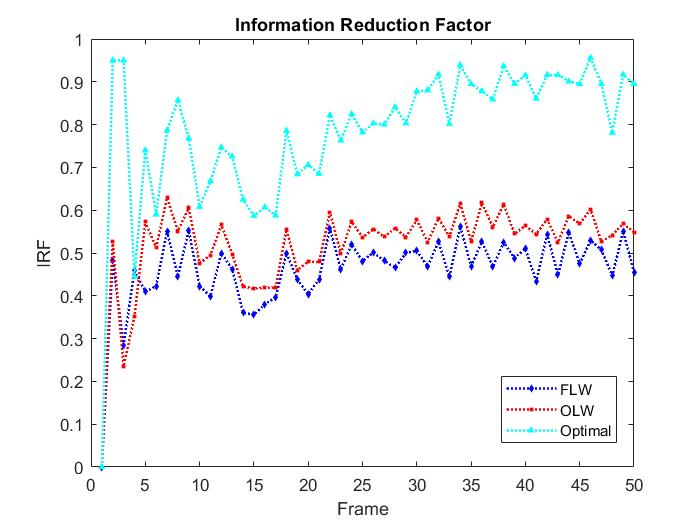
\includegraphics[scale=0.36]{IRF.jpg}
	\caption{Information reduction factor}
	\label{fig:IRF}
\end{figure}


\subsection{Performance of the Multitarget Tracker}
The optimal beam scheduler offers a higher IRF and thus, a lower PCRLB. However, PCRLB is only a theoretically lower bound and may not be achieved in real-life cases. In practice, we are more concerned with the actual estimation error of the tracker.

The performance of the multitarget tracker is evaluated by the worst-case RMSE

\begin{equation}
	\text{RMSE}_k = \max_{q}\left[\frac{1} {N_{MC}}\sqrt{\sum_{j=1}^{N_{MC}}\left[\left(x_{q}^{k}-\hat{x}_{q}^{k,j}\right)^{2}+\left(y_{q}^{k}-\hat{y}_{q}^{k,j}\right)^{2}\right]} \right]
\end{equation}

%The tracker, along with the task scheduler, are independent of the beam scheduling algorithm. However, due to different IRFs obtained by different beam schedulers, errors may accumulate and in return affect the result of the task scheduler and the tracker. During the numerical simulations, situations occurred where the task scheduler made different decisions when working with different beam schedulers.

Fig. \ref{fig:Worst RMSE} shows the worst-case RMSE of all three tracks, along with the PCRLB offered by the optimal beam scheduler. With the optimal beam scheduler, the tracker has actual smaller estimation errors. 
Table \ref{tab:RMSE} gives the worst-case RMSE at selected time intervals. 

\begin{figure}
	\centering
	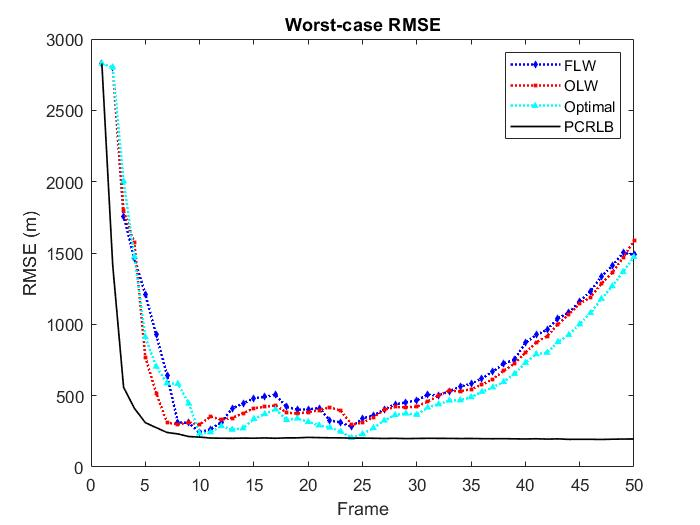
\includegraphics[scale=0.36]{Worst RMSE.jpg}
	\caption{Worst-case RMSE}
	\label{fig:Worst RMSE}
\end{figure}

\begin{table*}
	
	\centering
	
	\caption{Worst-case RMSE of Target Position Estimation}
	\begin{tabular}{cccc}
		\toprule
		\multirow{2}{*}{Time Index}&
		\multicolumn{3}{c}{Worst-case Position RMSE (m)}\cr
		\cmidrule(lr){2-4}
		&FLW&OLW&Optimal\cr
		\midrule
		5 & 1210.3 & \bf{508.2} & 961.9 \cr
		15 & 481.5 & 392.3 & \bf{387.4} \cr
		25 & 341.1 & 257.2 & \bf{235.5}  \cr
		\bottomrule
	\end{tabular}
	\label{tab:RMSE}
\end{table*}


Note that the number of radars is smaller than the number of targets, so there will be targets whose state and covariance are only predicted by the tracker but not updated due to missed measurements. At time $k=1$, since target 2 has the least PCRLB and therefore, not being tracked, its state will only be predicted and the error from the motion model is preserved, so the worst-case estimation error remains high.

The RMSE of target 3 is presented in Fig. \ref{fig:RMSE3}, which shows a better convergence than the worst-case RMSE.

\begin{figure}
	\centering
	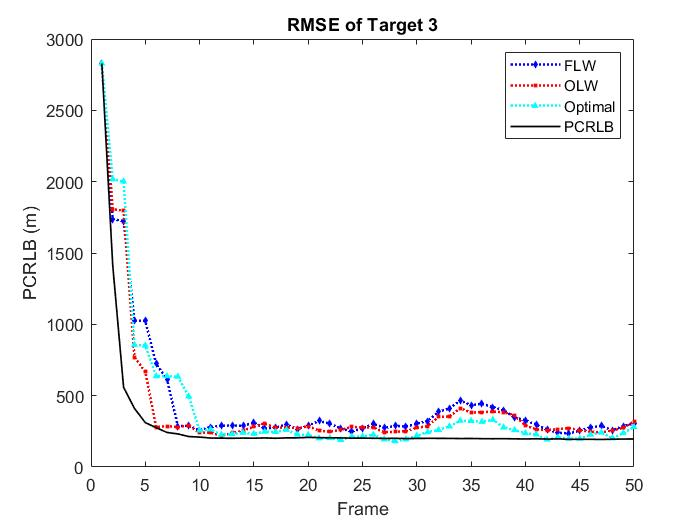
\includegraphics[scale=0.36]{RMSE3.jpg}
	\caption{RMSE of target 3}
	\label{fig:RMSE3}
\end{figure}

\subsection{Evaluation of algorithm speed}
To evaluate the efficiency of proposed algorithms, each algorithm's run time was recorded. All simulations are conducted using MATLAB R2019a on a laptop with a Core\texttrademark\ i5 2.6 GHz CPU and 8 GB RAM.

 \begin{table}
	\centering
	\caption{Average Time Cost}
	\begin{tabular}{cccc}
		\toprule
		Strategy & FLW & OLW & Optimal\\ 
		\midrule
		Time spent per frame (s) & 0.0042 & 1.2181 & 0.5462\\ 
		\bottomrule
	\end{tabular}
	\label{tab:Run time}
\end{table}

Table \ref{tab:Run time} gives the average time cost of the three algorithms. Due to hierarchical structure of HGA, beam scheduler 2 takes considerably longer time. It can be fastened by decreasing the population size and the maximum number of generation. Furthermore, intelligent operations can be utilized to reduce the time of defficient evolution, e.g., eliminating groups with low average fitness. 

Though the optimal solution takes less time than beam scheduler 2, its computational cost is still high compared with real-time requirements. In practical, sub-optimal strategies may be adopted to save time budget.

\section{Conclusion}
We addressed an adaptive beam scheduling problem for cooperative phased array radars. With the adoption of small-bandwidth pencil beams, the assumption that a beam can cover the potential location of targets no longer holds. Therefore, a more precise beam scheduler that controls the steering direction and operation time of the radar beam needs to be  developed. In this paper, we proposed two optimization models and  developed three solution strategies. The concept of expected PCRLB is proposed and the predictive EPCRLB is adopted as a criterion to minimize. Numerical simulations are presented. Results show that the optimal beam scheduler offers a lower worst-case PCRLB and the tracker working with it has a smaller estimation error.

This work can be further extended by considering the following issues. First, the scheduling of wide fan-beams can be jointly considered by adding the performance metrics of target detection into the optimization. Second, one can explore the simultaneous multibeam (SM) working mode of PARs where a PAR can simultaneously launch multiple beams. In this working mode, the issue of power allocation that determines how much power a radar assigns to each beam can be incorporated into the resource management problem.

\bibliographystyle{IEEEtran}
\bibliography{reference}
\end{document}